\documentclass[11pt]{article}

\usepackage{url}
\usepackage{multicol}
\usepackage[english]{babel}
\usepackage[margin=1in]{geometry}
\usepackage{graphicx}
\usepackage{subcaption}
\usepackage{enumitem}
\usepackage{amsmath}
\usepackage{amssymb}
\usepackage{wasysym}
\usepackage{color}
\usepackage{float}
\usepackage{nomencl}
\usepackage[title]{appendix}
\makenomenclature
\usepackage{pdfpages}
\usepackage{algorithm}
\usepackage{algpseudocode}
\usepackage{hyperref}
\hypersetup{
    colorlinks=true,
    linkcolor=blue,
    filecolor=magenta,      
    urlcolor=cyan,
    pdftitle={Overleaf Example},
    pdfpagemode=FullScreen,
    }
\title{16-745 Optimal Control Lecture 18}
\author{Reid Graves} 

\begin{document}
\maketitle

\section*{Last Time}
\begin{itemize}
    \item Stochastic Optimal Control
    \item LQG
\end{itemize}

\section*{Today}
\begin{itemize}
    \item  Optimal Estimation
    \item Finish LQG
    \item Duality
\end{itemize}

\section{From Last time}
\begin{itemize}
    \item ``Certainty Equivalence"
    \item ``Separation Principle"
    \item Frequently applied to nonlinear systems in practice
\end{itemize}

\section{Optimal State Estimation}
\begin{itemize}
    \item What should I optimize
    \begin{figure}[H]
        \centering
        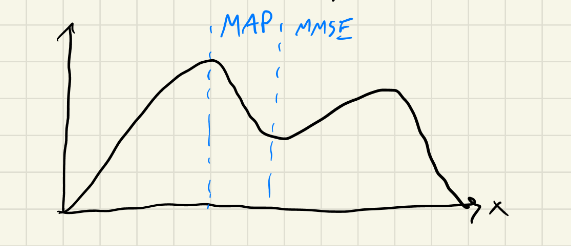
\includegraphics[width=0.5\linewidth]{lecture_20_1.png}
    \end{figure}
    \item Maximum a-posterior: (MAP)
    \begin{align*}
        \text{argmax}  \underbrace{p(x|y)}_{\textcolor{cyan}{\text{probability of state given measurements}}}
    \end{align*}
    \item Minimum mean squared error (MMSE)
    \begin{align*}
        &\text{arg}\min_{\hat{x}}\quad E[(x-\hat{x})^T(x-\hat{x})] \quad\textcolor{cyan}{\text{``Least squares" or ``minimum variance"}}
        \\
        &E[tr((x-\hat{x})^T(x-\hat{x}))] = E[tr((x-\hat{x})(x-\hat{x})^T)]\textcolor{cyan}{\text{ Changed from inner product to outer product (Covariance matrix) }\Sigma}
        \\
        &= tr(E[(x-\hat{x})(x-\hat{x})^T]) = tr(\Sigma)
    \end{align*}
    \item These are the same for a Gaussian!
\end{itemize}

\section{Kalman Filter}
\begin{itemize}
    \item Recursive linear MMSE estimator
    \item AsSigmae an estimate of the state that includes all measurements up to the current time:
    \begin{align*}
        \hat{x}_{k|k} &= E[x_k|y_{1:k}]
    \end{align*}
    \item AsSigmae we also know the error covariance:
    \begin{align*}
        \Sigma_{k|k} &= E[(x_k-\hat{x}_{k|k})(x_k-\hat{x}_{k|k})^T]
    \end{align*}
    \item We want to update $\hat{x}$ and $\Sigma$ to include a new measurement at $t_{k+1}$
    \item the KF can be broken into 2 steps
\end{itemize}

\subsection{Prediction}
\begin{align*}
    \hat{x}_{k+1|k} &= E[Ax_k + Bu_k + w_k|y_{1:k}] = A\hat{x}_{k|k} + Bu_k
    \\
    \Sigma_{k+1|k} &= E[(x_{k+1}-\hat{x}_{k+1:k})(\dots)^T]
    \\
    &= E[(Ax_k + Bu_k +w_k - A\hat{x}_{k|k} - Bu_k)(\dots)^T]
    \\
    &= A\underbrace{E[(x_k-\hat{x}_{k|k})(\dots)^T]}_{\textcolor{cyan}{\Sigma_{k|k}}} A^T + \underbrace{E[w_kw_k^T]}_{\textcolor{cyan}{W}}
    \\
    &= A\Sigma_{k|k}A^T + W \quad(\textcolor{cyan}{x_k\text{ and }w_k \text{ are encorrelated}})
\end{align*}
\subsection{Measurement Update}
\begin{itemize}
    \item Define ``innovation"
    \begin{align*}
        z_{k+1} &= y_{k+1} - C\hat{x}_{k+1|k} 
        \\
        &= Cx_{k+1} + v_{k+1} - C\hat{x}_{k+1|k}
    \end{align*}
    \item Innovation Covariance 
    \begin{align*}
        S_{k+1} &= E[z_{k+1}z^T_{k+1}]
        \\
        &= E[(Cx_{k+1} + v_{k+1} - C\hat{x}_{k+1|k})(\dots)^T] 
        \\
       & \textcolor{cyan}{*\text{ }v_{k+1}\text{ and } x_{k+1}\text{ are uncorrelated}}
       \\
       & \Rightarrow S_{k+1} = C\underbrace{E[(x_{k+1}-\hat{x}_{k+1|k})(\dots)^T]}_{\textcolor{cyan}{\Sigma_{k+1|k}}}C^T + \underbrace{E[v_{k+1}v_{k+1}^T]}_{\textcolor{cyan}{V}}
       \\
       &= C\Sigma_{k+1|k}C^T + V
       \end{align*}
       \item Innovation is the error signal we feed back into the estimator
       \item State Update:
       \begin{align*}
           \hat{x}_{k+1|k+1} &= \hat{x}_{k+1|k} + \underbrace{L_{k+1}}_{\textcolor{cyan}{1}}z_{k+1}
           \\
           &\textcolor{cyan}{1: \text{``Kalman Gain"}}
       \end{align*}
       \item Covariance Update
        \begin{align*}
            \Sigma_{k+1|k+1} &= E[(x_{k+1}-\hat{x}_{k+1})(\dots)^T]
            \\
            &= E[(x_{k+1}-\hat{x}_{k+1|k}-L_{k+1}((x_{k+1}+ v_{k+1} - (\hat{x}_{k+1|k}))(\dots)^T]
            \\
            &\textcolor{cyan}{* v_{k+1} \text{ and } x_{k+1} \text{ are uncorrelated}}
            \\
            &= \underbrace{(I-L_{k+1}C)\Sigma_{k+1|k}(I-L_{k+1}C)^T + L_{k+1}VL_{k+1}^T}_{\textcolor{cyan}{\text{``Joseph Form"}}}
        \end{align*}
       \item Kalman Gain
       \begin{align*}
           &MMSE \Rightarrow \text{minimize } E[(x_{k+1}-\hat{x}_{k+1|k+1})^T(\dots)]
           \\
           &E[(x_{k+1}-\hat{x}_{k+1|k+1})^T(\dots)] = tr\left(\Sigma_{k+1|k+1}\right)
       \end{align*}
       \begin{align*}
           \Rightarrow & \text{set }\frac{\partial tr(\Sigma_{k+1|k+1})}{\partial L_{k+1}}= 0 \quad(\text{ and solve for }L_{k+1})
       \end{align*}
       \begin{align*}
           \boxed{L_{k+1 = \Sigma_{k+1|k}C^TS_{k+1}^{-1}}}
       \end{align*}
\end{itemize}

\section{Kalman Filter Algorithm Summary}
\begin{enumerate}
    \item Start with $\hat{x}_{0|0}, \Sigma_{0|0}, W, V$
    \item Predict:
    \begin{align*}
        \hat{x}_{x+1|k} &= A\hat{x}_{k|k} + Bu_k
        \\
        \Sigma_{k+1_k} &= A\Sigma_{k|k}A^T + W
    \end{align*}
    \item Calculate Innovation + Covariance:
    \begin{align*}
        z_{k+1} &= y_{k+1} - C\hat{x}_{k+1|k}
        \\
        S_{k+1} &= C\Sigma_{k+1|k} C^T + V
    \end{align*}
    \item Calculate Kalman Gain:
    \begin{align*}
        L_{k+1} &= \Sigma_{k+1|k} C^TS_{k+1}^{-1}
    \end{align*}
    \item Update
    \begin{align*}
        \hat{x}_{k+1|k+1} &= \hat{x}_{k+1|k} + L_{k+1}Z_{k+1} \\
        \Sigma_{k+1|k+1} &= (I-L_{k+1}C)\Sigma_{k+1|k}(I-L_{k+1}C)^T + L_{k+1}VL_{k+1}^T
    \end{align*}
    \item GoTo 2
\end{enumerate}

\section{How do we apply this to nonlinear systems?}
\begin{itemize}
    \item Extended KF: Linearize abount $\hat{x}$ and proceed as in standard KF
    \item Many other generalizations
\end{itemize}

\section{Duality and Trajectory Optimization}
\begin{itemize}
    \item MMSE estmation problem is equivalent to the following optimal control problem:
    \begin{align*}
        &\min_{x_{1:N},w_{1:N}}\sum_{k=1}^{N-1}\frac{1}{2}\underbrace{(y_k - g(x_k))^TV^{-1}(y_k-g(x_k)}_{\textcolor{cyan}{\text{state cost}}} + \underbrace{\frac{1}{2}w_k^TW^{-1}w_k}_{\textcolor{cyan}{\text{control cost}}}
        \\
        & \quad s.t. \quad x_{k+1} = f(x_k) + w_k\leftarrow \textcolor{cyan}{\text{controls}}
        \\
        &g(x_k):\textcolor{cyan}{\text{ Measurement model}}
    \end{align*}
    \item If $f(x) = Ax$ and $g(x) = Cx$, this is an LQR problem
\end{itemize}


\end{document}
